Nahezu alle Datenschutzmechanismen für E-Mails sind erst wesentlich später als die ursprünglichen Protokolle wie SMTP entstanden und haben sich mit der Zeit entwickelt. Viele der vorgestellten Technologien sind unabhängige Lösungen, die lediglich in Verbindung mit E-Mail Systemen verwendet werden können, andere sind wiederum Protokollerweiterungen, die sich mehr oder weniger sinnvoll in das Gesamtkonzept einfügen. Sichtbar anhand der untersuchten Technologien ist allerdings, dass hier keine konsistente Lösung vorliegt. Jede Lösung zielt auf einen anderen Bereich ab und versucht ein atomares Problem zu lösen, ohne dabei auf die Kohärenz eines in der Praxis eingesetzten E-Mail Systems achten zu können. Dies öffnet unabhängig vom Kohärenzproblem auch das Problem der Konfiguration eines konkreten Systems. Die immense Komplexität der zusammenspielenden Komponenten wurde in Kapitel 1 erhellt und ist ein praktisches Problem solcher Systeme.

Dennoch ist es möglich die genannten Systeme zu nutzen, um eine Reihe von Problemen bezüglich Datensicherheit zu lösen. Um die Inhaltsdaten des Bodies einer E-Mail für jeden außer der Empfängerperson unzugänglich zu machen, kann das asymmetrische Verschlüsselungsverfahren GPG benutzt werden. Selbst der Server-Betreiber oder ein Man-in-the-Middle ist dann nicht in der Lage, die E-Mail ohne weiteres zu entschlüsseln, unabhängig davon, in welcher Weise diese transportiert wurde. Allerdings bezieht sich GPG nur auf den Body einer E-Mail und nicht auf die Header. Ebenso ist es möglich, die Protokoll-Transaktionen von SMTP, POP3 und IMAP über direktes TLS oder STARTTLS zu verschlüsseln. Problematisch hierbei ist aber, dass eine verschlüsselte Verbindung nicht durchgängig garantiert werden kann, z.b. wenn die Verbindung über mehrere MTAs geht oder wenn der E-Mail Server erlaubt zu unverschlüsselten Verbindungen herunterzustufen, insbesondere über SMTP STARTTLS. Und letzten Endes ist eine gewisse Anonymisierung der IP-Verbindungsdaten über TorBirdy möglich. Diese gilt allerdings nur für die Kommunikation des MUA mit dem MSA bzw. POP3/IMAP server.

\autoref{fig:bewertung} zeigt sehr deutlich, dass selbst beim Einsatz all dieser Technologien und unter der Voraussetzung korrekter Konfiguration immer noch eine wesentliche Stelle nicht ausreichend anonymisiert oder verschlüsselt werden kann. Dies ist nämlich die Kommunikation zwischen mehreren MTAs. Hier kann durchgängig nicht angenommen werden, dass Transaktionen verschlüsselt sind. Ebenso sind die Verbindungen direkt und weiterleitende E-Mail Server werden über den \verb#Received# Header gekennzeichnet. Somit ist es ohne viel Aufwand möglich, den Weg, den eine E-Mail nimmt, nachzuverfolgen und zumindest die kommunizierenden E-Mail Server eindeutig zu bestimmen. Die Menge an offenen Metadaten an dieser Stelle ist so hoch, dass hier keine Gesamtlösung zu erkennen ist und u.U. Sender und Empfänger direkt identifiziert werden können.

Allerdings ist festzuhalten, dass abgesehen von der mangelnden Verschleierung der Kommunikation zwischen MTAs, die existierenden Technologien die Basis einer Gesamtlösung bilden können.

\begin{figure}[htb]
	%\Centerfloat
	\centering
	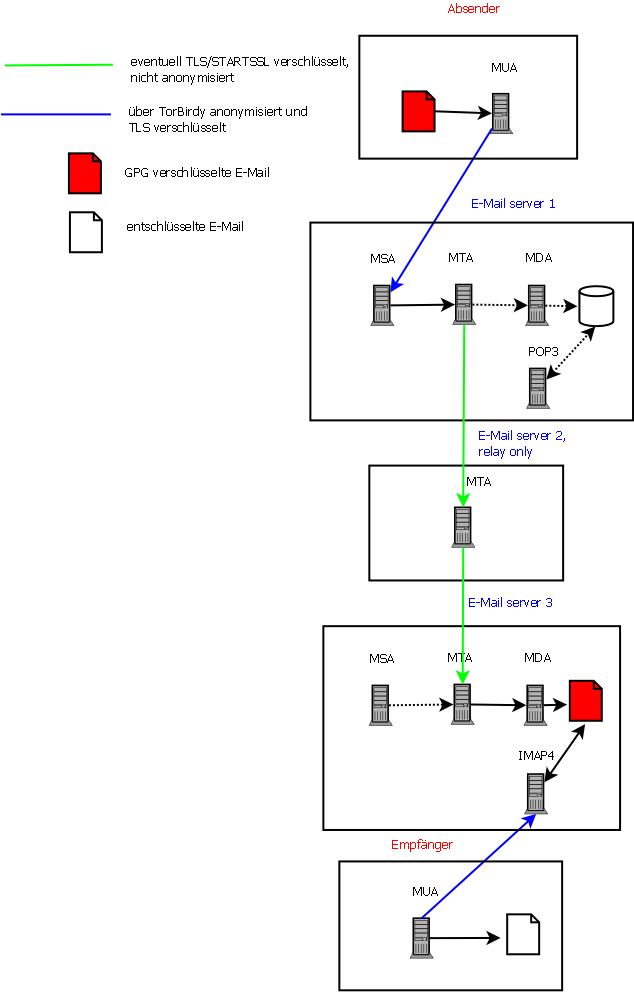
\includegraphics[scale=0.4]{Content/Problematik/BetrachtungDatenschutz/Bewertung.png}
	\caption{Übersicht Datenschutz in E-Mail Systemen}
	\label{fig:bewertung}
\end{figure}
\vfill
\clearpage

